\documentclass{beamer}
\usetheme[block=fill]{metropolis}

\usepackage[english]{babel}
\usepackage[utf8]{inputenc}

% For notes
\usepackage{pgfpages}
\setbeameroption{show notes on second screen=right}
\usepackage{appendixnumberbeamer} % don't number the backup slides

\usepackage{amsmath,amssymb} % math
\usepackage{graphicx} % images
\DeclareGraphicsExtensions{.eps,.pdf,.png,.jpg,.gif}
\graphicspath{{./img/}}

\title{aursec - Master a blockchain approach to securing software packages}
\author{Lukas Krismer \& Bennett Piater}
\institute{Universität Innsbruck - QE - Christian Sillaber}
\date{\today}

\begin{document}

\maketitle

\begin{frame}
	\frametitle{Outline}
	\tableofcontents
\end{frame}

\section{AUR}

\begin{frame}{AUR}
\begin{itemize}
	\item AUR=Arch Linux Repository
	\item Contains package descriptions (PKGBUILDs)
	\item everybody can upload PKBUILDs
	\item 3 different Requests
	\item voting system
\end{itemize}
\note{Orphan,Deletion,Merge}
\end{frame}

\begin{frame}{Threats}
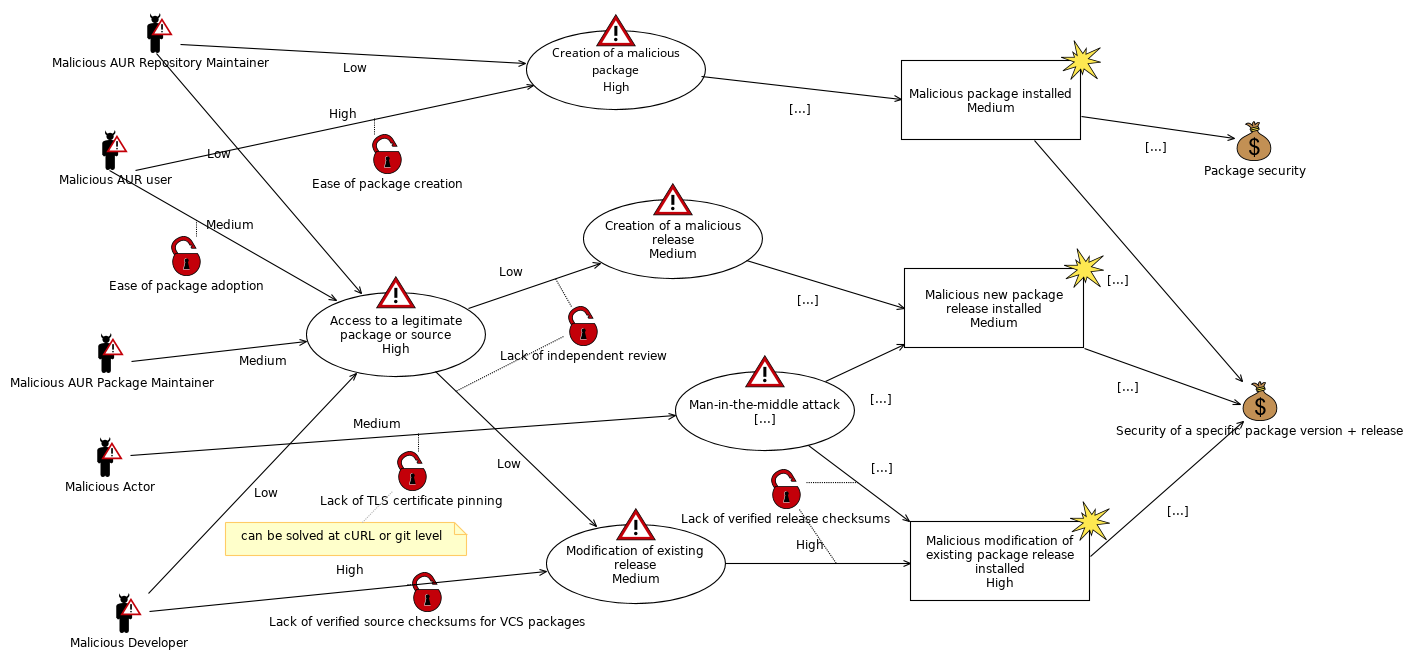
\includegraphics[width=\textwidth]{threat.png}
\note{}
\end{frame}

\section{Our Project}

\begin{frame}{Covered Threats}
\includegraphics<1>[width=\textwidth]{threat.png}
\includegraphics<2>[width=\textwidth]{threat.png} %TODO: change to reworked threatdiag.
\end{frame}

\begin{frame}{Basic Workflow}
%\icludegraphics[width=\textwidth]{bennets.diagram}
\end{frame}

\begin{frame}{Components}
\begin{itemize}
	\item Ethereum program
	\item libary
	\item arch-package
	\item web- and/or CLI-Interface
	\item integration
\end{itemize}

\end{frame}

\begin{frame}{Schedule}
\begin{itemize} 
	\item \textbf{25.10} Prototype hashing \hfill B
	\item \textbf{08.11} Inital-Presentation\hfill L
	\item \textbf{15.11} Libary-prototyp without blockchain-backend \hfill B/L
	\item \textbf{15.11} Bash-API for the blockchain \hfill L
	\item \textbf{30.11} Solidity-program finished \hfill B
	\item \textbf{08.12} unified local libary for development \hfill L
	\item \textbf{08.12} runnable server with ethereum-node \hfill B/L
	\item \textbf{15.12} libary-backend \hfill L
	\item \textbf{20.12} contrib: rudimentary pre-build-hooks in aurutils \hfill B
\end{itemize}
\end{frame}

\begin{frame}{Schedule}
\begin{itemize} 
	\item \textbf{10.01} contrib: TLS-public-key-pinning in aurutils \hfill B
	\item \textbf{10.01} configuration and trust-cutoff \hfill L
	\item \textbf{15.01} testing: integration in aurutils \hfill B
	\item \textbf{15.02} arch-package inc. private blockchain \hfill B
	\item \textbf{01.03} finish: libary and aurutils-Hook \hfill B
	\item \textbf{01.04} finish: Web- and/or CLI-Interface \hfill L
	\item \textbf{15.04} draft paper \hfill 
	\item \textbf{??.05} finish: paper\hfill 
	\item \textbf{??.05} End-Presentation\hfill L
\end{itemize}
\end{frame}


\end{document}
